\documentclass[a4paper,11pt]{article}
\usepackage[T1]{fontenc}
\usepackage[utf8]{inputenc}
\usepackage{lmodern}
\usepackage{graphicx}
\usepackage[top=2cm, bottom=2cm, left=2cm, right=2cm]{geometry}

\title{INFO-F-404~: Real-Time Operating Systems\\Project 1~: Audsley}
\author{Rémy Detobel, Stanislas Gueniffey and Denis Hoornaert}

\begin{document}

\maketitle

\section{Implementation choices}
  The aim of the present section is to give to the reader a quick overview of the utility of each of the implemented classes.\\
  
  \begin{figure}[ht!]
    \centering
    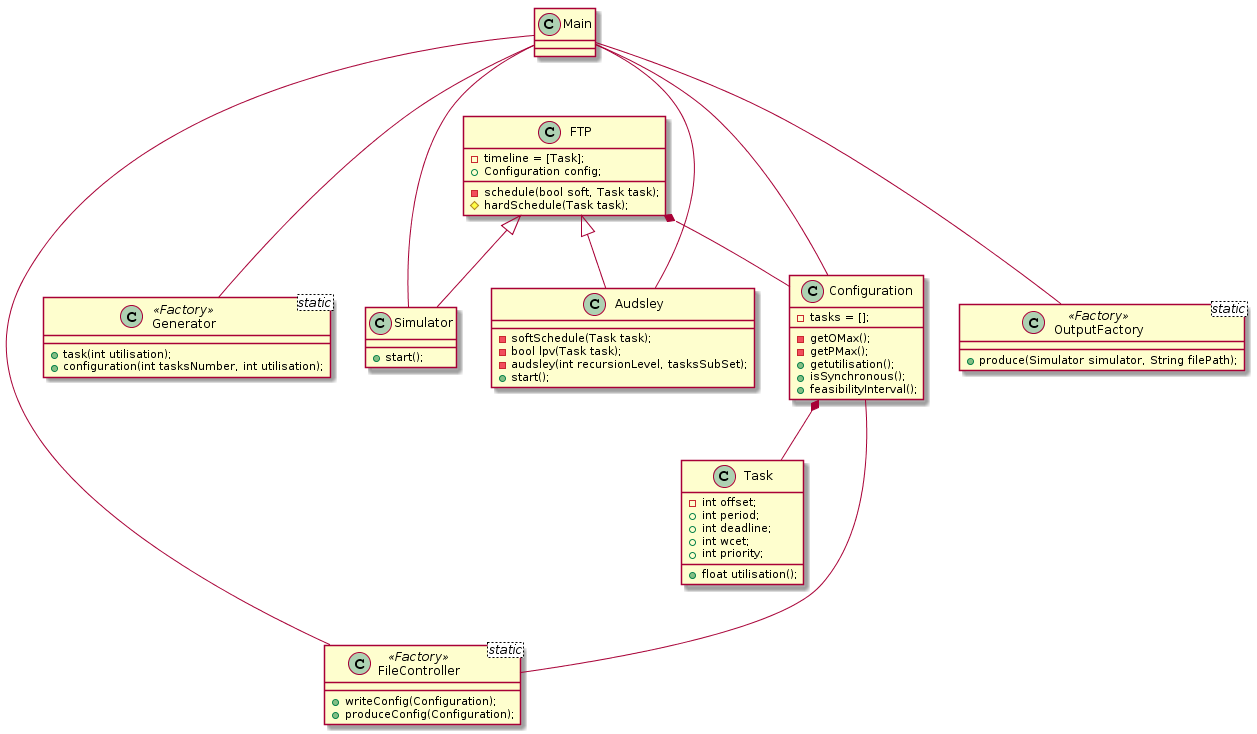
\includegraphics[scale=0.175]{img/uml.png}
    \caption{Pseudo-uml of the project}
    \label{fig:pseudo-uml}
  \end{figure}
  \noindent The project is composed of various classes. Among these classes, some are elementary as they are used in every aspect of the project (e.g. \verb|Configuration|) whereas the others are specific to a feature (e.g. \verb|Generator|).\\
  
  \noindent The "elementary" classes~:
  \begin{itemize}
    \item \verb|Configuration|~: This object is produce by the \verb|FileController| class and, similarly to the theory, is mainly a set/collection of tasks. The class also provides useful methods used throughout the project by other classes (e.g. \verb|isSynchronous()|).
    \item \verb|Tasks|~: This class can simply be seen as a bunch of useful data (close from the theory : nothing less-nothing more).
  \end{itemize}
  The "scheduling dedicated" classes~:
  \begin{itemize}
    \item \verb|FTP|~: Abbreviation of Fixed Task Priority, this class just regroup common features of its two children (\verb|Simulator| and \verb|Audsley|). Typically, these features are the time line structure, the hard scheduling and so on.
    \item \verb|Simulator|~: The class has for only objective to hard schedule every tasks of a given \verb|Collection| object and to print the "events" of the simulation as stipulated in the assignment statement.
    \item \verb|Audsley|~: Even though this class inherits from \verb|FTP| like \verb|Simulator|, its objective is different as it does not aim to simulate anything. In fact, this class is focused on computing the \textit{least priority viable task} of a tasks collection and deducing a adequate priority assignment using the Audsley algorithm.
  \end{itemize}
  There are three Factory classes~:
  \begin{itemize}
    \item \verb|FileController|~: This class is dedicated to the reading and the writing of tasks collection from and to a file.
    \item \verb|OutputFactory|~: The aim of this class is to encapsulate the mechanism used to generate a visual representation of a scheduling (For further information see \ref{sec:output-dependencies}).
    \item \verb|Generator|~: As ask in the assignment statement, the project should be able to generate a task collection given two parameters. IN our project, the class \verb|Generator| is the class that achieves this feature.
  \end{itemize}

\section{Difficulties encountered}
  One of the difficulties encountered during the realisation of the project is the generation of random systems. More precisely : how to ensure that the utilisation of the generated system is as close as possible to the utilisation specified by the user ?\\
  The issue has been addressed as follow~:\\
  By definition, the total utilisation of the system is given by~:
  \[U(\tau)=\sum\limits_{i}^{n}U(\tau_{i}) \hspace{2cm} U(\tau_{i})=\frac{C_{i}}{T_{i}}\]
  Where~:
  \begin{itemize}
    \item $n$ is the number of tasks specified by the user
    \item $U(\tau)$ is the total utilisation of the system specified by the user
  \end{itemize}
  We generate a vector of size $n$ for which each cell contains a random integer $i \in [10, 100]$. This vector is supposed to be the vector of tasks utilisation. Thus, we compute the factor by which each cell has to be divided so that the sum is equal to the desired utilisation.
  \[U(\tau)=\frac{\sum_{i}^{n}rand(i)}{factor} \hspace{1cm} \Leftrightarrow \hspace{1cm} factor=\frac{\sum_{i}^{n}rand(i)}{U(\tau)}\]
  For example~:
  \[rand = [30, 40, 50, 60],~|rand| = 4,~U(\tau)=70\]
  \[factor = \frac{30+40+50+60}{70} \approx 2.57\]
  \[utilisations = [11.67, 15.56, 19.46, 23.35]\]
  Once done, we can create a task based on the given utilisation (one of the vector) as follow~:
  \begin{enumerate}
    \item we generate a random offset
    \item we generate a random WCET with the condition that it must be greater than 0 because otherwise the task is useless and because a negative wcet makes no sense
    \item for the period, we cannot generate a fully random value as the utilisation must be respected. Hence, we determine its value using the following formula~:
      \[U(\tau_{i}) = \frac{C_{i}}{T_{i}} \hspace{1cm} \Leftrightarrow \hspace{1cm} T_{i} = \frac{C_{i}}{U(\tau_{i})}\]
    \item we generate a random deadline with the condition that it must at least be equal to the wcet and at most equal to the period
  \end{enumerate}
  Applying this process, implies the use of a lot of float numbers and the approximations that comes with. However, we still manage to have a nice total utilisation approximation.
  \begin{figure}[h!]
    \centering
    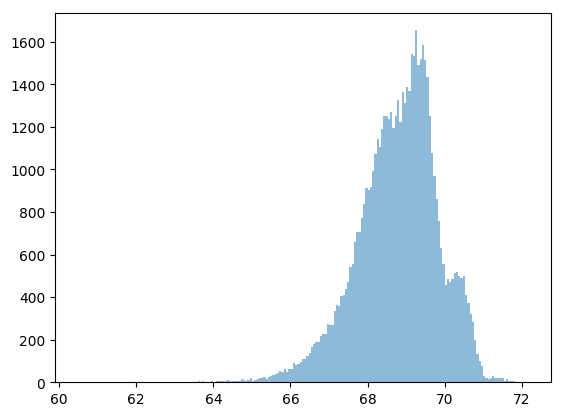
\includegraphics[scale=0.7]{img/distribution.png}
    \caption{Distribution of utilisation of generated systems (6 tasks with a targeted $70\%$ of utilisation)}
  \end{figure}

\section{Project output dependencies}
  \label{sec:output-dependencies}
  The python modules used to generate the image of the scheduling are called \verb|numpy| and \verb|matplotlib|. Even though they are quite famous amongst python programmers, they are not part of the standard library. Hence, they need to be manually installed sometimes. This can be easily be achieved by using \verb|pip3| and by typing the following commands~:
  \begin{verbatim}
sudo pip3 install numpy
sudo pip3 install matplotlib
  \end{verbatim}
  The commands above have been tested on Ubuntu 16.04 LTS but might differ depending on the distribution and the version.\\
  
  \noindent Important~: The code will only produce an image if the user append the name of the desired image file to the command used for starting a simulation. If no fourth argument is provided then a simple simulation will be executed. Example~:
  \begin{verbatim}
    python3 project.py sim <start> <stop> <taskFile> <imageFile>
  \end{verbatim}
  \begin{figure}[ht!]
    \centering
    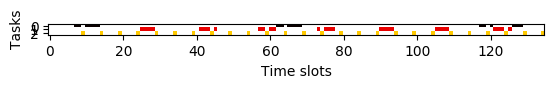
\includegraphics{img/schedule1.png}
    \caption{An example of an image generated by the project}
    \label{fig:scheduling-output-example}
  \end{figure}

\end{document}
